\documentclass[fleqn,a4paper,12pt]{article}

%used Packages
\usepackage{standalone}		% Zum Einlesen aus anderen .tex-Files
\usepackage{geometry}		% Zur Bearbeitung des Layouts (Ränder,...)
\usepackage[german]{babel}
\usepackage[utf8]{inputenc}
\usepackage{amsmath}		% Mathematische Symbole
\usepackage{amssymb}     	% Nochmehr mathematische Symbole
\usepackage{dsfont}      	% Schriftsatz fuer Zahlenmengensymbole
%\usepackage{verbatim}   	% erweiterte Verbatim-Umgebung
\usepackage{alltt}       	% Quasi-Verbatim-Umgebung
\usepackage{fancyhdr}    	% Eigene Kopfzeilen
\usepackage{graphicx}    	% Zum Einbinden von Grafiken
							% Einbinden einer eps-Grafik geht so: includegraphics{path}
\usepackage{wrapfig}
\usepackage{lscape}
\usepackage{rotating}
\usepackage{epstopdf}

% Skalierung der Grafiken
\setlength{\unitlength}{1cm}

\frenchspacing               % Kein Extrafreiraum nach Satzzeichen
\setlength{\parindent}{0pt}  % Neue Absaetze nicht einruecken
%\sloppy                     % Schlampige Absatzformatierung
\fussy                       % Penible Absatzformatierung
\linespread{1.5}             % Zeilenabstand


% Seitenraender
\geometry{left=30mm, right=40mm, bottom=30mm}
				% Doc-class, Packageimports, fancy stuff
%%Seitenränder formatieren
\addtolength{\voffset}{-2cm}
\addtolength{\textheight}{0cm}
\addtolength{\hoffset}{0cm}
\addtolength{\textwidth}{2cm}
\addtolength{\headheight}{2cm} % fuer jeden Strichkode einen Zentimeter

% Font fuer Code 39
\font\xlix=wlc39 scaled 1200
\newcommand\barcode[1]{{\xlix@#1@}}

% Name, Matrikelnummer, Barcode
\newcommand\student[2]{
	\mbox{\scriptsize
		\begin{tabular}{@{}l@{}r@{}}
			\multicolumn{2}{@{}r@{}}{\barcode{#2}}\\
			#1&#2\\
		\end{tabular}}}

% Kopfzeile
\pagestyle{fancy}            % Eigene Kopfzeilen verwenden
\lhead{
	\small
	\textsc{Grundlagen der Signalverarbeitung \\
		WS 2017/2018 \\
		\"Ubung (\today)}
	\vfill}
\rhead{
	\begin{tabular}[b]{@{}rr@{}}
		\student{Philipp Badenhoop}{572693} &
		\student{Steven Lange}{568733} \\
		\student{Pascal Jochmann}{575056} &
		\student{Kevin Trogant}{572451}
\end{tabular}}			% Definition der Kopfzeile
%andere Definitionen
\providecommand{\R}{{\mathbb R}}
\providecommand{\N}{{\mathbb N}}
\providecommand{\Z}{{\mathbb Z}}
\providecommand{\Q}{{\mathbb Q}}
\providecommand{\C}{{\mathbb C}}
\providecommand{\F}{\mathcal{F}}
\providecommand{\less}{\setminus}
\providecommand{\inv}{{}^{-1}}
\providecommand{\Land}{\bigwedge}
\providecommand{\Lor}{\bigvee}			% Liste der zusätzlichen Commands und redefines

\begin{document}
	\begin{landscape}
	\section*{Übungsaufgabe 19:}
	a) \newline
	\begin{tabular}{c c | c c c c c c c }
			& n	& 0	& 1	& 2	& 3 & 4 & 5 \\
		\cline{2-9}
			& $t_n$	& -3 & -2 & 0 & 1 & 2 & 3 \\
			& $f_n$	& 9 & 4	& 0	& 1 & 4 & 9 \\
		m & $\varphi_m$	& &	& &	& & & $\sum_{n=0}^{N-1}$\\
		\cline{1-9}	
		0 & $cos(0)$ & 1 & 1 & 1 & 1 & 1 & 1 & 6\\
		1 & $cos(t)$ & $cos(-3)$ & $cos(-2)$ & 1 & $cos(1)$ & $cos(2)$ & $cos(3)$ & -1.27\\
		2 & $cost(2t)$ & $cos(-6)$ & $cos(-4)$ & 1 & $cos(2)$ & $cos(4)$ & $cos(6)$ & 1.2 \\
		\cdashline{1-9}
		& $cos(t) \cdot cos(2t)$ & $cos(-3) \cdot cos(-6)$ & $cos(-2) \cdot cos(-4)$ & 1 & $cos(1) \cdot cos(2)$ & $cos(2) \cdot cos(4)$ & $cos(3) \cdot cos(6)$ & -0.58 \\
		& $cos(t)^2$ & $cos(-3)^2$ & $cos(-2)^2$ & 1 & $cos(1)^2$ & $cos(2)^2$ & $cos(3)^2$ & 3.6\\
		& $cos(2t)^2$ & $cos(-6)^2$ & $cos(-4)^2$ & 1 & $cos(2)^2$ & $cos(4)^2$ & $cos(6)^2$ & 3.87\\
	\end{tabular} \newline \newline
	Mit der folgenden Gleichung
	\begin{align*}
		\left(\begin{matrix}
			a_{00}	&	\dots	& a_{0,m-1}\\
			\vdots	&			& \vdots\\
			a_{m-1,0}	&	\dots	& a_{m-1,m-1}
		\end{matrix}\right)\cdot \left(\begin{matrix}c_0\\\vdots\\c_{m-1}\end{matrix}\right) = 
		\left(\begin{matrix}
			\sum_{n=0}^{N-1} \varphi_0(t_n)\cdot f(t_n)\\
			\vdots\\
			\sum_{n=0}^{N-1} \varphi_{m-1}(t_n)\cdot f(t_n)\\
		\end{matrix}\right)
	\end{align*}
	mit $a_{i,j}:= \sum_{n=0}^{N-1}\varphi_i(t_n)\cdot \varphi_j(t_n)$ ergibt sich daraus:
	\begin{align*}
		\left(\begin{matrix}c_0\\c_1\\c_2\end{matrix}\right) = 
		\left(\begin{matrix}
			6 &	-1.27 & 1.2\\
			-1.27 & 3.6 & -0.58\\
			1.2 &	-0.58 & 3.87
		\end{matrix}\right)^{-1} \cdot
		\left(\begin{matrix}
			1\\
			5.29\\
			3.37\\
		\end{matrix}\right) \approx 
		\left(\begin{matrix}
			0.33\\
			1.75\\
			1.03
		\end{matrix}\right)
	\end{align*}
	Damit ergibt sich für $f_{app}(t) = 1.03 \cdot cos(2t)+1.75 \cdot cos(t)+0.33 \cdot cos(0)$ folgendes Fehlermaß
	\begin{align*}
		E^2(c) = \sum_{i=0}^5 \left[ f(t_n) - f_{app}(t_n)\right]^2 = 17.93
	\end{align*}
	
	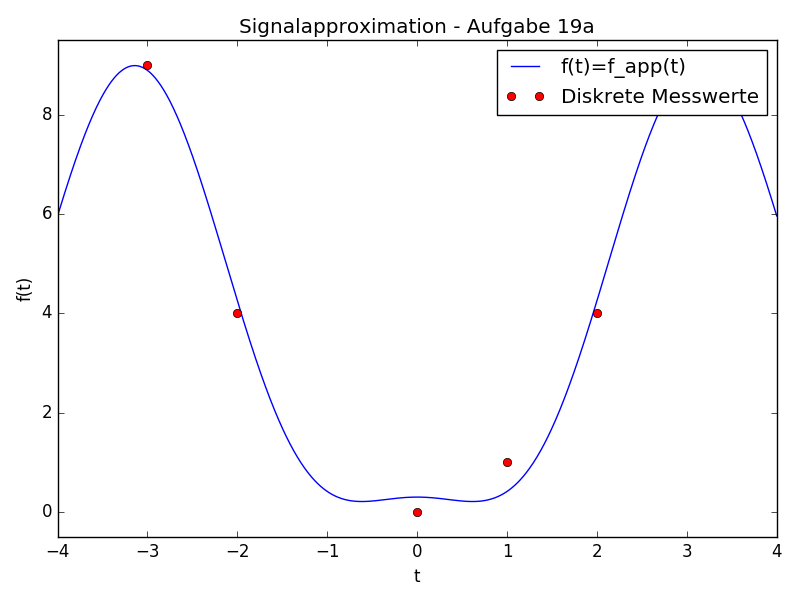
\includegraphics[scale=0.4]{A19a.png}
	\end{landscape}
\end{document}